\chapter{Opis projektnog zadatka}


\textnormal{Ideja i cilj ovoga projekta je napraviti web aplikaciju za košarkaški klub Rudeš, odnosno razviti programsku podršku za istu.
	Iako navedeni klub trenutno već posjeduje svoje web stranice koje omogućuju neke osnovne mogućnosti i funkcionalnosti, one su
	izrađene korištenjem vrlo jednostavnog programa (WYSIWYG Web Builder) u kojemu se nudi mogućnost izrade web stranice najobičnijom 
	i relativno jednostavnom drag 'n' drop metodom. Upravo zbog tog razloga sadašnja web stranica košarkaškog kluba Rudeš nema nikakav
	backend, kao ni bazu podataka, odnosno ne posjeduje nikakve karakteristike ili značajke zbog kojih bi se mogla nazvati pravom web 
	aplikacijom. Također, mnoge funkcionalnosti koje su naizgled omogućene, ipak nisu implemetirane i tako zasigurno pogoršavaju iskustvo 
	korisnika prilikom korištenja same stranice (na primjer, na stranici postoji nekoliko gumba na čiji bi se pritisak trebale otvoriti 
	stranice koje vode do određenog sadržaja, međutim, sadržaja tamo često nema). Osim toga, sam dizajn stranice je nespretno izveden i 
	zasigurno bi se mogao poboljšati kako bi korisnicima izgledao atraktivnije. Link na trenutnu stranicu jest \url{https://www.kkrudes.hr}
	Takve web stranice posjeduju još neki klubovi kao npr. KK Cedevita, s veoma malim razlikama kao što su nepostojanje Live Streaminga ili web shop koji ide preko neke druge stranice.
}

\bigbreak

\textnormal{Osnovni motiv ovoga projekta je promijeniti navedena obilježja web stranice i čitavi site zapravo napraviti ispočetka, ni iz čega.
	Međutim, ovoga puta sa svim jasno istaknutim funkcionalnostima koje su klubu potrebne i koje unaprijeđuju i obogaćuju doživljaj
	korisnika kojemu je ona namijenjena za korištenje.
	Prilikom pokretanja same aplikacije vidljiva je početna stranica kluba gdje se nalazi naslovna traka s rubrikama koje omogućuju 
	pregled nekih osnovnih informacija. Između ostalog, tu se korisniku pruža mogućnost prijave u sustav. Korisnik se može prijaviti 
	postojećim računom, za koji mu je potreban email i lozinka. Osim toga, korisniku se nudi opcija registracije novim računom.}

\pagebreak

\textnormal{Ukoliko korisnik nije registriran, omogućen mu je pristup sljedećim sadržajima:}
\begin{packed_item}
	\item pregled igrača
	\item pregled utakmica
	\item pregled kontakta kluba
	\item pregled novosti vezanih uz klub
	\item pregled webshopa
	\item dodavanje artikala u košaricu
\end{packed_item}

\textnormal{Ipak, neregistrirani korisnik ne može obavljati kupovinu. Upravo po tome se razlikuje od registriranog korisnika kojemu je ta opcija dozvoljena.}
\textnormal{Za registraciju korisnika potrebno je sljedeće:}
\begin{packed_item}
	\item korisničko ime
	\item lozinka
	\item e-mail adresa
	\item ime
	\item prezime
\end{packed_item}
\textnormal{ Za prijavu u sustav nije potreban broj kartice, kao ni broj mobilnog telefona, no može se dodati prilikom kupnje u webshopu. Korisnik
	koji je registriran može mijenjati svoj račun ili ga obrisati. Neregistrirani korisnik registracijom postaje klijent.}
\bigbreak
\underline{\textit{Klijent} }\textnormal {je korisnik koji, osim što ima sve ovlasti kao i neregistrirani korisnik, dodatno može gledati prijenos utakmica uživo i obaviti kupovinu u webshopu.
	Klub posjeduje svoje hoodice, majice i dresove koji se mogu naručiti, odnosno kupiti. Klijent u webshopu stavlja u košaricu artikle koje 
	želi i ima namjeru kupiti. Ukoliko se klijent odluči kupiti određeni proizvod, prosljeđuje ga se do plaćanja gdje se transakcija izvršava.
	Tada se obaviještava uprava.
	Klijent u webshopu može ocjenjivati artikle, birati veličine i dodavati te mijenjati informacije o plaćanju kreditnom karticom. Također, može uključiti obavijesti da mu se na e-mail kojim se registrirao šalju novosti o novodostupnim artiklima i popustima u webshopu. Kako košarkaški klub Rudeš ponekad prenosi svoje utakmice uživo na YouTubeu, aplikacija bi nudila dio rezerviran za streaming koji
	je povezan s YouTubeom i omogućuje prijavljenim korisnicima gledanje utakmica uživo, odnosno prijenosa. S desne strane prijenosa 
	nalazi se prilagodeni chat u kojem korisnici mogu komunicirati za vrijeme prijenosa. Dok nema prijenosa, u dijelu rezerviranom za 
	prijenose pišu informacije o idućoj utakmici ili prijenosu, što je poznato unaprijed.}
\bigbreak
\textnormal {Među registriranim korisnicima postoje još 2 tipa korisnika, a to su administrator aplikacije te treneri, odnosno uprava kluba.}
\bigbreak
\underline{\textit{Treneri kluba} }\textnormal {su zaduženi za kreiranje sadržaja web aplikacije. U sadržaj ubrajamo slike, novosti te podatke kluba.  Također imaju ovlasti upravljanja igračima, odnosno mogu mijenjati njihove podatke.}
\bigbreak
\underline{\textit{Uprava kluba, tj. članovi uprave}} \textnormal {imaju ovlasti za dodavanje i mijenjanje artikla u webshopu. Imaju na uvid koliko je veličina pojedinih artikala ostalo te ih mogu dodavati, mijenjati cijene, dodavati popuste ili brisati.}
\bigbreak
\textit{\underline{Administrator  aplikacije} }\textnormal {je korisnik s najvećim ovlastima. On ima potpuni pristup bazi podataka i može brisati i dodavati trenere. Ima
	sve ovlasti kao i treneri/uprava kluba, s dodatkom da može nekoga od trenera ili uprave proglasiti administratorom. Može i brisati 
	recenzije koje nisu u skladu s pravilima aplikacije.}
\bigbreak
\textnormal{Aplikacija je lokalizirana na hrvatski i engleski jezik. Sustav podržava rad više korisnika u stvarnom vremenu.}
\textnormal{Stranica će biti javno objavljena te će ju moći koristiti bilo tko s pristupom internetu.
	Korist ovog projekta je u tome da će stranicu koristiti sadašnji i budući članovi košarkaškog kluba Rudeš. Jedna od mogućih nadogradnji
	jest lokaliziranje aplikacije na njemački jezik te dodavanje foruma za raspravu o košarkaškim, a i ostalim temama širokog spektra.}





% \section{Primjeri u LaTeXu}

% \textit{Ovo potpoglavlje izbrisati.}\\

% U nastavku se nalaze različiti primjeri kako koristiti osnovne funkcionalnosti LaTeXa koje su potrebne za izradu dokumentacije. Za dodatnu pomoć obratiti se asistentu na projektu ili potražiti upute na sljedećim web sjedištima:
% \begin{itemize}
% 	\item Upute za izradu diplomskog rada u LaTeXu - \url{https://www.fer.unizg.hr/_download/repository/LaTeX-upute.pdf}
% 	\item LaTeX projekt - \url{https://www.latex-project.org/help/}
% 	\item StackExchange za Tex - \url{https://tex.stackexchange.com/}\\

% \end{itemize} 	



% %Ovo poglavlje je potrebno prilikom predaje obrisati

% \underbar{podcrtani tekst}, 
% \textbf{podebljani tekst}, 
% \textit{nagnuti tekst}\\
% \normalsize primjer
% \large primjer
% \Large primjer
% \LARGE {primjer}
% \huge {primjer}
% \Huge primjer
% \normalsize

% \begin{packed_item}

% 	\item  primjer
% 	\item  primjer
% 	\item  primjer
% 	\item[] \begin{packed_enum}

% 		\item primjer
% 		\item primjer
% 	\end{packed_enum}

% \end{packed_item}

% \noindent primjer url-a: \url{https://www.fer.unizg.hr/predmet/opp/projekt}


% \begin{longtabu} to \textwidth {|X[8, l]|X[8, l]|X[16, l]|} %definicija sirine polja

% 	\hline \multicolumn{3}{|c|}{\textbf{naslov unutar tablice}}	 \\[3pt] \hline
% 	\endfirsthead

% 	\hline \multicolumn{3}{|c|}{\textbf{naslov unutar tablice}}	 \\[3pt] \hline
% 	\endhead

% 	\hline 
% 	\endlastfoot

% 	\rowcolor{LightGreen}IDKorisnik & INT	&  	Lorem ipsum dolor sit amet, consectetur adipiscing elit, sed do eiusmod  	\\ \hline
% 	korisnickoIme	& VARCHAR &   	\\ \hline 
% 	email & VARCHAR &   \\ \hline 
% 	ime & VARCHAR	&  		\\ \hline 
% 	\cellcolor{LightBlue} primjer	& VARCHAR &   	\\ \hline 


% \end{longtabu}


% \begin{table}[H]



% 	\begin{longtabu} to \textwidth {|X[8, l]|X[8, l]|X[16, l]|} %definicija sirine polja

% 		\hline 
% 		\endfirsthead

% 		\hline 
% 		\endhead

% 		\hline 
% 		\endlastfoot

% 		\rowcolor{LightGreen}IDKorisnik & INT	&  	Lorem ipsum dolor sit amet, consectetur adipiscing elit, sed do eiusmod  	\\ \hline
% 		korisnickoIme	& VARCHAR &   	\\ \hline 
% 		email & VARCHAR &   \\ \hline 
% 		ime & VARCHAR	&  		\\ \hline 
% 		\cellcolor{LightBlue} primjer	& VARCHAR &   	\\ \hline 


% 	\end{longtabu}

% 	\caption{\label{tab:referencatablica} Naslov ispod tablice.}
% \end{table}

% \begin{figure}[H]
% 	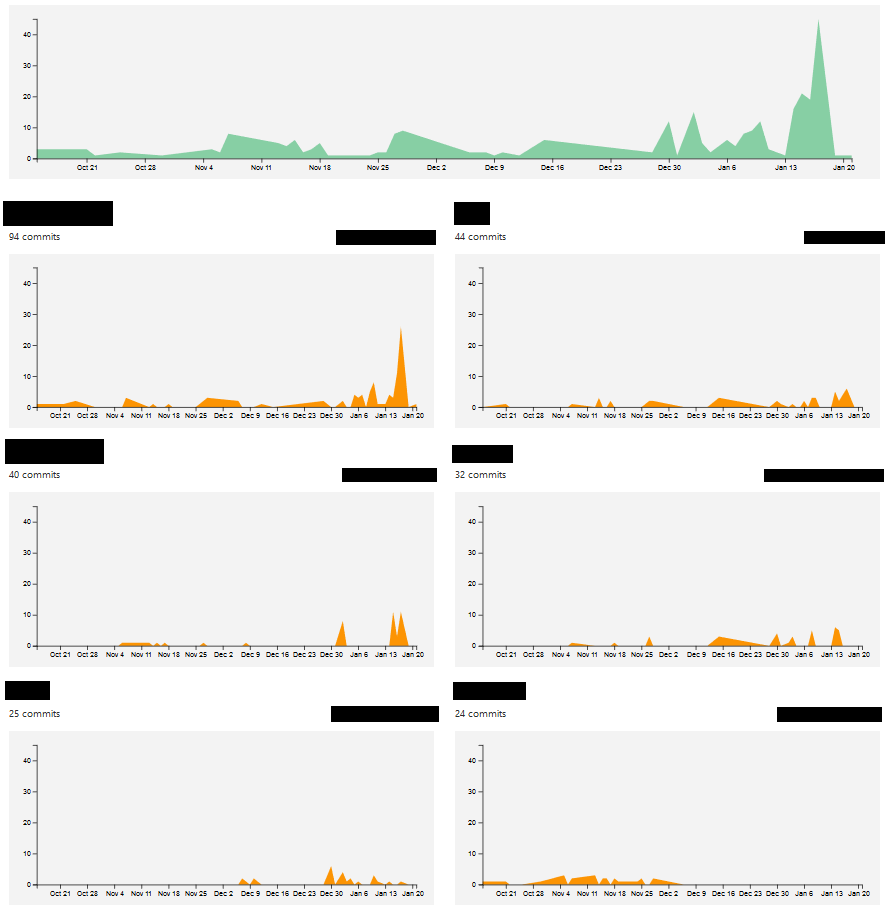
\includegraphics[scale=0.4]{slike/aktivnost.PNG}
% 	\centering
% 	\caption{Primjer slike s potpisom}
% 	\label{fig:promjene}
% \end{figure}

% \begin{figure}[H]
% 	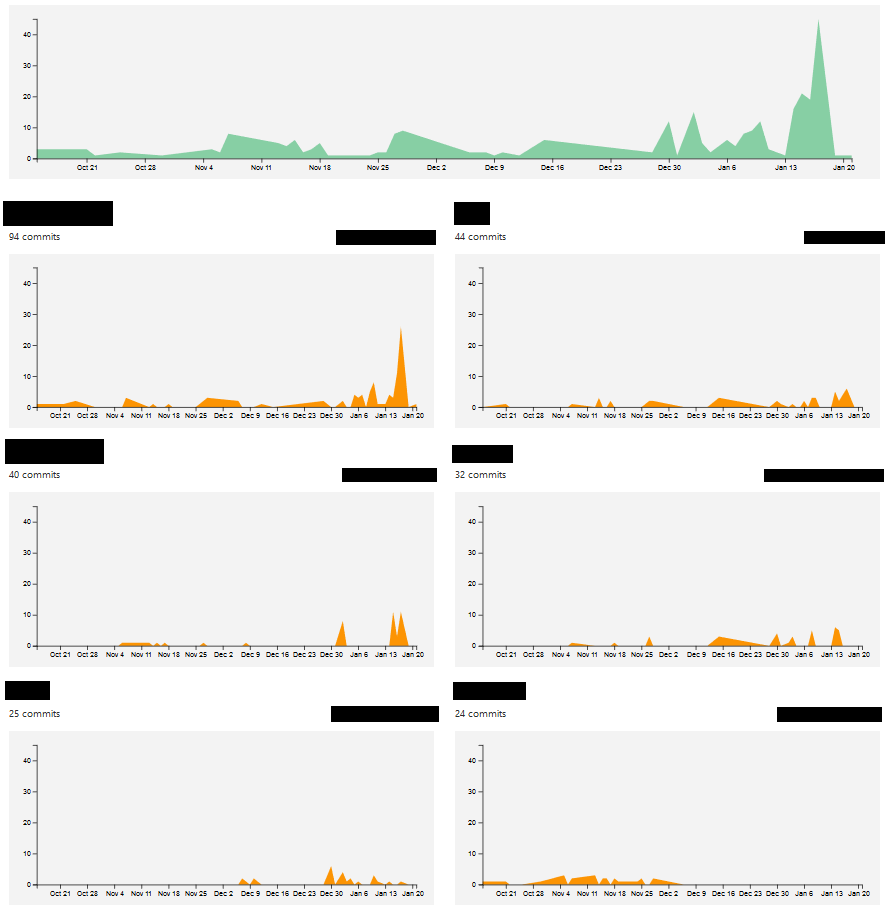
\includegraphics[width=\linewidth]{slike/aktivnost.PNG}
% 	\caption{Primjer slike s potpisom 2}
% 	\label{fig:promjene2}
% \end{figure}



\eject

